\newpage
\subsection{Restaurant management}
\begin{enumerate}
    \item Use-case diagram:
    \begin{center}
        \begin{figure}[!h]
            \begin{center}
                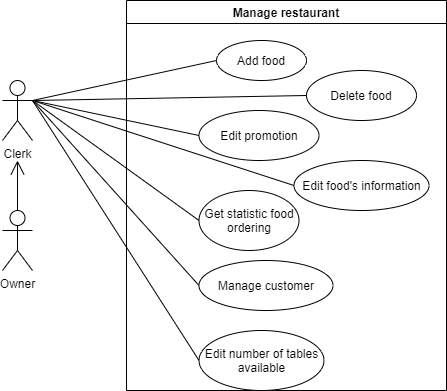
\includegraphics[scale=.5]{Images/managementDiagram.png} 
            \end{center} 
            \vspace{1cm}
            \caption{Restaurant management's use-case diagram}
        \end{figure}    
    \end{center}
    
    \item Use-case "Delete food":
    \begin{center}{\color{black}}
        \begin{tabular}{|p{5cm}|p{7cm}|} \hline
            Tên usecase &   Delete food\\ \hline
            Actor& Clerks \\ \hline
            Mô tả& Use-case cho phép nhân viên có thể xóa món ăn có trong menu \\ \hline
            Tiền điều kiện &    
            \begin{enumerate}[1.]
                \item Nhân viên đã đăng nhập vào hệ thống
                \item Nhân viên chọn chức năng xóa món ăn
            \end{enumerate}\\ \hline
            Hậu điều kiện & Món ăn đã được xóa thành công \\ \hline
            Luồng sự kiện chính &  
                \begin{enumerate}[1.]
                    \item Hệ thống hiển thị màn hình các món ăn có thể xóa.
    				\item Nhân viên chọn món ăn cần xóa.
    				\item Nhân viên chọn hoàn thành
    				\item Hệ thống thông báo đã xóa thành công
    				\item kết thúc use-case
                \end{enumerate}\\
            \hline
        \end{tabular}
    \end{center}
    
    \newpage
    \item Use-case "Add food":
    \begin{center}{\color{black}}
        \begin{tabular}{|p{5cm}|p{7cm}|} \hline
            Tên usecase &   Add food\\ \hline
            Actor& Clerks \\ \hline
            Mô tả& Use-case cho phép nhân viên thêm món ăn mới vào trong menu \\ \hline
            Tiền điều kiện &
            \begin{enumerate}[1.]
                \item Nhân viên đã đăng nhập vào hệ thống
                \item Nhân viên chọn chức năng thêm món ăn
            \end{enumerate}\\ \hline
            Hậu điều kiện & Món ăn mới đã được thêm vào menu\\ \hline
            Luồng sự kiện chính &  
                \begin{enumerate}[1.]
                    \item Hệ thống hiển thị màn hình chứa các thông tin cần điền để mô tả món ăn mới.
                    \item Nhân viên điền các thông tin cần thiết cho món ăn mới.
                    \item Nhân viên xác nhận thông tin món ăn mới và ấn hoàn thành hoặc chọn chỉnh sửa lại.
    				\item kết thúc use-case.
                \end{enumerate} \\\hline
            Luồng sự kiện phụ &
            \begin{enumerate}[1.]
                \item Nhân viên chọn chỉnh sửa lại thông tin món ăn mới.
                \item Nhân viên chỉnh sửa các thông tin món ăn bị sai.
                \item Nhân viên xác nhận thông tin món ăn và ấn hoàn thành.
            \end{enumerate}\\ \hline
        \end{tabular}
    \end{center}
    
    \newpage
    \item Use-case "Edit food'information":
    \begin{center}{\color{black}}
        \begin{tabular}{|p{5cm}|p{7cm}|} \hline
            Tên usecase &   Edit food'information\\ \hline
            Actor& Clerks \\ \hline
            Mô tả& Use-case cho phép nhân viên chỉnh sửa thong tin món ăn trong menu \\ \hline
            Tiền điều kiện &
            \begin{enumerate}[1.]
                \item Nhân viên đã đăng nhập vào hệ thống
                \item Nhân viên chọn chức năng chỉnh sửa món ăn
            \end{enumerate}\\ \hline
            Hậu điều kiện & Thông tin món ăn đã được chỉnh sửa\\ \hline
            Luồng sự kiện chính &  
                \begin{enumerate}[1.]
                    \item Hệ thống hiển thị màn hình chứa các món ăn có thể chỉnh sửa.
                    \item Nhân viên chọn món ăn cần chỉnh sửa.
                    \item Nhân viên chỉnh sửa các thông tin cần thiết cho món ăn.
                    \item Nhân viên xác nhận thông tin món ăn và ấn hoàn thành hoặc chọn chỉnh sửa lại.
    				\item kết thúc use-case.
                \end{enumerate} \\\hline
            Luồng sự kiện phụ &
            \begin{enumerate}[1.]
                \item Nhân viên chọn chỉnh sửa lại thông tin món ăn.
                \item Nhân viên chỉnh sửa các thông tin món ăn bị sai.
                \item Nhân viên xác nhận thông tin món ăn và ấn hoàn thành.
            \end{enumerate}\\ \hline
        \end{tabular}
    \end{center}
    
    \newpage
    \item Use-case "Edit promotion":
    \begin{center}{\color{black}}
        \begin{tabular}{|p{5cm}|p{7cm}|} \hline
            Tên usecase &   Edit promotion\\ \hline
            Actor& Clerks \\ \hline
            Mô tả& Use-case cho phép nhân viên đặt khuyến mãi cho món ăn\\ \hline
            Tiền điều kiện &    
            \begin{enumerate}[1.]
                \item Nhân viên đã đăng nhập vào hệ thống
                \item Nhân viên chọn chức năng thêm khuyến mãi.
            \end{enumerate}\\ \hline
            Hậu điều kiện & Thông tin khuyến mãi của món ăn đã được cập nhật\\ \hline
            Luồng sự kiện chính &  
                \begin{enumerate}[1.]
                    \item Hệ thống hiển thị màn hình các món ăn có thể đặt khuyến mãi.
    				\item Nhân viên chọn món ăn cần đặt khuyến mãi.
    				\item Nhân viên đặt giá khuyến mãi hoặc phần trăm khuyến mãi cho món ăn.
    				\item Nhân viên chọn hoàn thành
    				\item Hệ thống thông báo đã đặt khuyến mãi thành công.
    				\item kết thúc use-case
                \end{enumerate}\\
            \hline
        \end{tabular}
    \end{center}
    
    \item Use-case "get statistic food ordering":
    \begin{center}{\color{black}}
        \begin{tabular}{|p{5cm}|p{7cm}|} \hline
            Tên usecase &  Get statistic food ordering\\ \hline
            Actor& Clerks \\ \hline
            Mô tả& Use-case cho phép nhân viên thống kê về các đơn hàng đã được thực hiện \\ \hline
            Tiền điều kiện &
            \begin{enumerate}[1.]
                \item Nhân viên đã đăng nhập vào hệ thống
                \item Nhân viên chọn chức năng lấy thống kê đơn hàng
            \end{enumerate}\\ \hline
            Hậu điều kiện &     Người dùng biết được thống kê các đơn hàng đã được thực hiện\\ \hline
            Luồng sự kiện chính &  
                \begin{enumerate}[1.]
                    \item Hệ thống hiển thị màn hình chứa các thống kê về số lượng các đơn hàng, tổng thu, thông tin cụ thể các đơn hàng.
    				\item kết thúc use-case
                \end{enumerate} \\\hline
        \end{tabular}
    \end{center}
    
    \item Use-case "Manage customer":
    \begin{center}{\color{black}}
        \begin{tabular}{|p{5cm}|p{7cm}|} \hline
            Tên usecase & Manager customer\\ \hline
            Actor& Clerks \\ \hline
            Mô tả& Use-case cho phép nhân viên thống kê các thông tin về các khách hàng \\ \hline
            Tiền điều kiện &
            \begin{enumerate}[1.]
                \item Nhân viên đã đăng nhập vào hệ thống
                \item Nhân viên chọn chức năng quản lí khách hàng.
            \end{enumerate}\\ \hline
            Hậu điều kiện & Nhân viên biết được các thông tin về các khách hàng \\ \hline
            Luồng sự kiện chính &  
                \begin{enumerate}[1.]
                    \item Hệ thống hiển thị màn hình chứa các thông tin về số lượng các khách hàng của hệ thống, các thông tin của từng khách hàng.
    				\item kết thúc use-case
                \end{enumerate} \\\hline
        \end{tabular}
    \end{center}
    
    \item Use-case edit number of tables available:
    \begin{center}{\color{black}}
        \begin{tabular}{|p{5cm}|p{7cm}|} \hline
            Tên usecase &   Edit number of tables available\\ \hline
            Actor& Clerks \\ \hline
            Mô tả& Use-case cho phép nhân viên chỉnh sửa số bàn có thể đặt giữ chỗ của nhà hàng\\ \hline
            Tiền điều kiện &
            \begin{enumerate}[1.]
                \item Nhân viên đã đăng nhập vào hệ thống
                \item Nhân viên chọn chức năng chỉnh sửa số bàn dành cho đặt trước.
            \end{enumerate}\\ \hline
            Hậu điều kiện &     Nhân viên cài đặt số bàn có thể đặt thành công \\ \hline
            Luồng sự kiện chính &  
                \begin{enumerate}[1.]
                    \item Hệ thống hiển thị màn hình chỉnh sửa số bàn mà khách có thể giữ chỗ
                    \item Nhân viên nhập số bàn: Bàn vip, bàn cho gia đình, bàn cho couple. 
                    \item Nhân viên chọn chọn hoàn thành
    				\item kết thúc use-case
                \end{enumerate} \\\hline
        \end{tabular}
    \end{center}
\end{enumerate}